\documentclass{article}
\usepackage{amsfonts}
\usepackage{amsmath}
\usepackage[letterpaper, top=0.75in, left=0.75in, right=0.75in, bottom=0.89in]{geometry} % for custom margins
\usepackage{fancyhdr} % for headers
\usepackage{graphicx} % for including images
\usepackage{caption} % for captions
\usepackage[shortlabels]{enumitem}
\usepackage{float}
% Define headers and footers
\DeclareMathOperator*{\argmin}{argmin}
\pagestyle{fancy}
\fancyhf{}
\usepackage{algorithm}
\usepackage{algpseudocode}
\usepackage{bm}
% Left header
\fancyhead[L]{MTE544 Fall 2024}

% Center header
\fancyhead[C]{Assignment\#2}

% Right header
\fancyhead[R]{Due Nov.\ 8\textsuperscript{th} 11:59 \textsc{PM}}
\fancyfoot[C]{\thepage}
\begin{document}

\section{RANSAC with Ellipse I (18)}

In this exercise, you are tasked to detect an ellipse based on given dataset using RANSAC.
\begin{figure}[H]
    \centering
    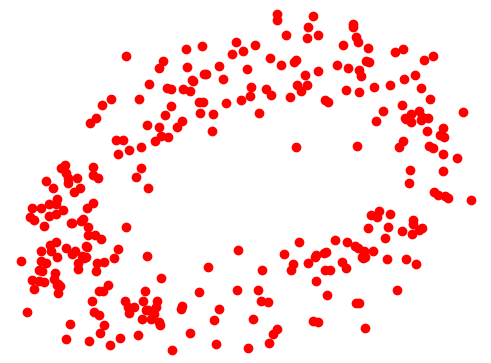
\includegraphics[width=0.65\textwidth]{img/ellipse.png}
    \caption{A Plot of Randomly Selected Dataset}
    \label{fig:p3c1}
\end{figure}
The goal is to estimate the parameters $\mathbf{Q}$ and $\mathbf{b}$ by fitting the sensor data to an ellipse. 
An ellipse can be described by the quadratic equation: 
\begin{equation*}
(\mathbf{p}-\mathbf{b})^\top\mathbf{Q}(\mathbf{p}-\mathbf{b})=1
\end{equation*}
or
\begin{equation*}
    Ax^2+2Bxy+Cy^2-2Dx-2Ey+1=0
\end{equation*}
where:
\begin{itemize}
\item $\mathbf{Q}=\mathbf{Q}^\top\in\mathbb{R}^{2\times2}$ is a unique symmetric positive definite matrix of coefficients. [If $\mathbf{Q}$ is not positive definite, you may have a hyperbola instead.]
\end{itemize}
Note that the coefficients ($A$,$B$,$C$,$D$,and $E$) are also unique.
The conversion from the polynomial coeffcients to the quadratic form can be expressed as follows:
\begin{equation*}
    \begin{aligned}
        \mathbf{Q}&=\alpha\begin{bmatrix}
        A & B\\ B & C
    \end{bmatrix}\\
    \mathbf{Q}\mathbf{b}&=\alpha\begin{bmatrix}
        D\\E
    \end{bmatrix}\\
    \alpha&=\frac{1}{\begin{bmatrix}
        D & E
    \end{bmatrix}\begin{bmatrix}
        A & B \\ B & C
    \end{bmatrix}^{-1}\begin{bmatrix}
        D \\ E
    \end{bmatrix}-1}
    \end{aligned}
\end{equation*}

\begin{enumerate}[a.)]  
\item Determine the minimum number of points to uniquely determined ellipse's parameters as well as derive a method to construct an ellipse with the parameters ($A$,$B$,$C$,$D$, and $E$) based on those points. $\mathbf{p}_i=(x_i,y_i)$ denote the $i^\text{th}$ data point. You must explain your rationale to receive credits. [10 pts]
\[\]
Answer:
The general form of an ellipse is:
\begin{equation*}
    Ax^2+2Bxy+Cy^2-2Dx-2Ey+1=0
\end{equation*}
From this equation, it is evident that with five unknowns, five points are needed to uniquely determine an ellipse's parameters.
Each point is written as:
\[
p_i = (x_i, y_i)
\]
Substituting \(x = x_i\) and \(y = y_i\) for \(i = 1, 2, 3, 4, 5\) into the ellipse equation.
This results in a system of five linear equations:
\[
\begin{cases}
A x_1^2 + B x_1 y_1 + C y_1^2 + D x_1 + E y_1 = 1 \\
A x_2^2 + B x_2 y_2 + C y_2^2 + D x_2 + E y_2 = 1 \\
A x_3^2 + B x_3 y_3 + C y_3^2 + D x_3 + E y_3 = 1 \\
A x_4^2 + B x_4 y_4 + C y_4^2 + D x_4 + E y_4 = 1 \\
A x_5^2 + B x_5 y_5 + C y_5^2 + D x_5 + E y_5 = 1 \\
\end{cases}
\]
Rewriting the above system of linear equations:
\[
\begin{bmatrix}
x_1^2 & x_1 y_1 & y_1^2 & x_1 & y_1 \\
x_2^2 & x_2 y_2 & y_2^2 & x_2 & y_2 \\
x_3^2 & x_3 y_3 & y_3^2 & x_3 & y_3 \\
x_4^2 & x_4 y_4 & y_4^2 & x_4 & y_4 \\
x_5^2 & x_5 y_5 & y_5^2 & x_5 & y_5 \\
\end{bmatrix}
\begin{bmatrix}
A \\ B \\ C \\ D \\ E
\end{bmatrix}
=
\begin{bmatrix}
1 \\ 1 \\ 1 \\ 1 \\ 1
\end{bmatrix}
\]
Solving:
\[
\begin{bmatrix}
A \\ B \\ C \\ D \\ E
\end{bmatrix}
=
\begin{bmatrix}
x_1^2 & x_1 y_1 & y_1^2 & x_1 & y_1 \\
x_2^2 & x_2 y_2 & y_2^2 & x_2 & y_2 \\
x_3^2 & x_3 y_3 & y_3^2 & x_3 & y_3 \\
x_4^2 & x_4 y_4 & y_4^2 & x_4 & y_4 \\
x_5^2 & x_5 y_5 & y_5^2 & x_5 & y_5 \\
\end{bmatrix}^{-1}
\begin{bmatrix}
1 \\ 1 \\ 1 \\ 1 \\ 1
\end{bmatrix}
\]
\item 
Fit an ellipse with the following datasets and compute for $\mathbf{Q}$, $\mathbf{b}$, $A$, $B$, $C$, $D$ and $E$.

\begin{equation*}
    (2.92, -6.01), \quad (3.40, -7.20), \quad (4.99, -7.84), \quad (5.48, -7.04), \quad (4.20, -5.91)
\end{equation*}

 You don't have code for this part, but you still have to do it with Python in the next part. [8 pts.]
\end{enumerate}

\newpage
\section{RANSAC with Ellipse II (30)}
In this exercise, you are tasked to implement RANSAC algorithm for determining the shape of an ellipse in Python. The implementation must match your explanation in the report in order to receive full credits.

To test whether point $\mathbf{p}_i$ is an inlier, let the following inequality be the condition for inliers.
\begin{equation*}
    \left\|\sqrt{(\mathbf{p}_i-\mathbf{b})^\top\mathbf{Q}(\mathbf{p}_i-\mathbf{b})}-1\right\|\leq \varepsilon
\end{equation*}
where $\varepsilon$ is the tunable threshold.
\begin{enumerate}[a.)]
\item Based on the given template in Python, implement \textit{fit\textunderscore ellipse\textunderscore subset} that compute $\mathbf{Q}$ and $\mathbf{b}$ from a given set of points. (The number points is determined from 1.a). [8 pts]

\item Based on the given template in Python, implement \textit{ransac\textunderscore ellipse} that determined the best $\mathbf{Q}$, $\mathbf{b}$, and the corresponding inliers based on the given dataset, number of iterations, and threshold. You must explain your implementation step-by-step [12 pts]
 with the rationale in your report.
\item Based on the given template in Python, use different number of dataset, number of iterations, and threshold value. Comment on the effect of these parameters. [10 pts]
\end{enumerate}
\newpage
\section{Differential-Drive Simulation [20 pts]}
Create a simulation for the 2WD robot with \underline{Python} which takes as inputs the linear and angular velocities $\begin{bmatrix}
    v,\omega
\end{bmatrix}^\top$ (you can use the state space form). You should obtain the poses of the robot $\begin{bmatrix}
    x(t),y(t),\theta(t)
\end{bmatrix}^\top$ as outputs. 
\begin{enumerate}[(a)]
    \item Simulate and plot the trajectories obtained for the following velocities (use at least 30 seconds with a timestep of 0.1s):
    \begin{enumerate}[i.]
        \item Constant velocities
        \begin{enumerate} [1.]
            \item $\begin{bmatrix}
    v,\omega
\end{bmatrix}^\top=\begin{bmatrix}
    1,0
\end{bmatrix}^\top$
\item $\begin{bmatrix}
    v,\omega
\end{bmatrix}^\top=\begin{bmatrix}
    0,0.3
\end{bmatrix}^\top$
\item $\begin{bmatrix}
    v,\omega
\end{bmatrix}^\top=\begin{bmatrix}
    1,0.3
\end{bmatrix}^\top$
        \end{enumerate}
        \item Velocity profiles: $\begin{bmatrix}
            v(t)\\\omega(t)
        \end{bmatrix}=\begin{bmatrix}
            1+0.1\cdot\sin(t)\\
            0.2+0.5\cdot\cos(t)
        \end{bmatrix}$
    \end{enumerate}
    Linear velocities are [m/s] and angular velocities are [rad/s]. For each case, plot the top view of the 2D trajectory ($x$ vs $y$), and then each variable against time, including orientation $\theta$. Discuss briefly your observations on the outcome (feel free to perform more tests). [15 pts]
    \item 	Assuming the robot has dimensions $T$ (track) $= 0.2$ [m], and wheel radius $r = 0.1$ [m], what are the wheel speeds $u_l$,$u_r$ needed to achieve the constant velocities in (a).i? 
    
    Briefly comment on how you would need to change your implemented simulation if instead of linear and angular velocities, the input control parameters were wheel speeds.


\end{enumerate}
\newpage
\section{ Bayesian Filter for Tracking Moo-Deng's Behavior II (20)}
In this exercise, you are tasked to implement a state estimator for Moo-Deng's whereabouts along with a simple behavior simulator in Python . The implementation must match your explanation in the report in order to receive full credits.
\begin{enumerate}[a)]
\item Based on the given code in Python, complete the function  \texttt{moodeng\textunderscore behavior\textunderscore update} that randomly returns the state of Moo-Deng based on the given current state and the transition matrix $\mathbf{A}$. 
You must explain your implementation in this report. Comment in the report on how can you use statistics to verify your results ? [5 pts.]

\textbf{Answer}: To verify the results of the completed function, the number of iterations can be increased to infinity (in practice, just a large number), after which the frequency of each state can be compared to $x^*$ from Question 3c.
\item Based on the given code in Python, complete the function \texttt{sensor\textunderscore measurement}  that return the noisy measurement $\mathbf{y}_k$ based on the matrix $\mathbf{C}$ and given Moo-Deng's state. Note that the results should be either (1,0,0), (0,1,0), or (0,0,1). [5 pts.]

\textbf{Answer}: See code provided
\item Based on the designed Bayesian filter and the given code in Python, implement a state estimator and the rest of the simulation in  called \texttt{sim\textunderscore moodeng}. The estimator should :
\begin{itemize}
    \item estimate a sequence state of Moo-Deng's location $\hat{A}_k$
    \item return a sequence belief (probability vector) of Moo-Deng's location $\mathbf{x}_k$
\end{itemize} 
given an initial belief $\mathbf{x}_0$ and a sequence of sensor measurement $\mathbf{y}_k$ [6 pts.]. 

\textbf{Answer}: See code provided
\end{enumerate}



\end{document}